\documentclass{article}

% if you need to pass options to natbib, use, e.g.:
% \PassOptionsToPackage{numbers, compress}{natbib}
% before loading nips_2016
%
% to avoid loading the natbib package, add option nonatbib:
% \usepackage[nonatbib]{nips_2016}

\usepackage[final]{nips_2016}

% to compile a camera-ready version, add the [final] option, e.g.:
%\usepackage[final]{nips_2016}

\usepackage[utf8]{inputenc} % allow utf-8 input
\usepackage[T1]{fontenc}    % use 8-bit T1 fonts
\usepackage{hyperref}       % hyperlinks
\usepackage{url}            % simple URL typesetting
\usepackage{booktabs}       % professional-quality tables
\usepackage{amsfonts}       % blackboard math symbols
\usepackage{nicefrac}       % compact symbols for 1/2, etc.
\usepackage{microtype}      % microtypography

\usepackage{bm}
\usepackage{amsmath}
\usepackage{amssymb}
\usepackage{layouts}
\usepackage{graphicx}

\newcommand{\mx}[1]{\mathbf{\bm{#1}}}

\title{Monaural speaker separation with supervised deep learning model using deep U-Net architecture and permutation invariant training -- Egycsatornás, beszélő szerinti hangszétválasztás felügyelt, permutáció-invariáns tanítású, U-Net felépítésű mély neurális hálóval}

% The \author macro works with any number of authors. There are two
% commands used to separate the names and addresses of multiple
% authors: \And and \AND.
%
% Using \And between authors leaves it to LaTeX to determine where to
% break the lines. Using \AND forces a line break at that point. So,
% if LaTeX puts 3 of 4 authors names on the first line, and the last
% on the second line, try using \AND instead of \And before the third
% author name.

\author{
  Dávid Besenyei \\
  Mechatronical Engineering BSc student\\
  Budapest University of Technology and Economics\\
  Budapest, Hungary \\
  \texttt{david.besenyei97@gmail.com} \\
  %% examples of more authors
  \And
  Zsolt Fischer \\
  Mechatronical Engineering BSc student\\
  Budapest University of Technology and Economics\\
  Budapest, Hungary \\
  \texttt{zsolt@fisu.hu} \\
  \And
  Donát Takács \\
  Mechatronical Engineering BSc student\\
  Budapest University of Technology and Economics\\
  Budapest, Hungary \\
  \texttt{takacs.donat01@gmail.com} \\
}

\begin{document}
% \nipsfinalcopy is no longer used

\maketitle

\begin{abstract}
This study presents a solution for the well-known speech separation problem. The execution is carried out by means of a deep neural network with U-Net structure. The problem of speech separation has a  rich literature. From the possible problems and difficulties, we present the case where two speakers' soundtracks are recorded by a single microphone. The goal of the project is to separate mixed speech and restore the audio channel of each original speaker.
\end{abstract}

\begin{abstracthu}
Jelen tanulmány egy U-Net struktúrájú mély neurális hálón alapuló beszédszeparációs megoldást mutat be. A beszédszeparáció problémája széles szakirodalommal rendelkezik. Az előforduló problémák közül azt az esetet mutatjuk be, ahol két beszélő hangsávjait egyetlen mikrofon rögzíti és a cél az összekevert beszéd szétválasztása a két beszélő szerint.
\end{abstracthu}

\section{Overview}

Speech separation is the task of separating
target speech from background interference. A special case of this task is multi-talker speaker-separation, where the interference is not noise, but an audio channel from another speaker. If there is only a single signal source available, the task is \textit{monaural speaker separation}. While this task was traditionally treated as a signal processing problem, recent developments in the field \cite{Wang14} allowed for the use of deep neural networks, mostly by formulating the problem as a classification problem, which is well-posed for usage with deep neural networks.

In a general multi-talker case, let us consider $S$ speakers, with \textit{clean audio signals} $\mx{x}_1,\, \mx{x}_2 ... \mx{x}_S$. The \textit{mixed signal} $\mx{y}$ is a composition of these signals. Thus the task of speaker separation is reversing this process: generating $\mx{x}_i$ from only $\mx{y}$. This is a problem that humans are quite good at solving: the so-called 'cocktail-party effect' can be observed by everyday life: in a noisy multi-talker environment, humans can successfully isolate and concentrate on the speech of a single individual. However, replicating this process using computers is still a very much open problem.

One recent, quite successful approach for treating this problem is the above-mentioned classification by deep neural networks. (An extensive, recent overview of state of the art results and practices in this field was published by Wang et al. in 2018 \cite{Wang18} which was used heavily during our work.) By calculating the (complex-valued) Short Time Fourier Transform (STFT) of the signals (denoted by $\mx{X}_i$ and $\mx{Y}$ respectively), time-frequency domain spectra can be obtained. By applying \textit{masks} $\mx{M}_i$ on the mixed $\mx{Y}$ spectrum, the original $\mx{X}_i$ channels are aimed to be obtained:
\begin{gather}
    \mx{X}_i = \mx{M}_i \circ \mx{Y}
\end{gather}
where $\circ$ denotes element-wise multiplication. However, since speaker-specific data is mostly contained in the magnitude values, a common approach is to use
\begin{gather}
    \left| \mx{X}_i \right| = \mx{M}_i \circ \left| \mx{Y} \right|
\end{gather}
in separation, and reconstruct $\mx{X}_i$ from the above magnitude and the phase of $\mx{Y}$:
\begin{gather}
    \mx{X}_i = \left| \mx{X}_i \right| \circ \mathrm{e} ^ {\mathrm{j}\ \mathrm{arg}\mx{Y}}
\end{gather}
where the power is element-wise and $\mathrm{j}$ is the imaginary unit.

This way, a deep neural network $h$ with parameters $\theta$ can be used to estimate masks for each speaker:
\begin{gather}
    \left\{  \hat{\mx{M}}_i \right\} = h( \left| \mx{Y} \right| ; \theta)
\end{gather}
which is indeed a classification problem: the network needs to estimate for each time-frequency value how much it belongs to each speaker. Often a softmax restriction is used on the masks (like in \cite{YuKTJ16}): $\sum_i^S \hat{\mx{M}}_i = \mx{I}$. While this is used for magnitude masks as well as complex masks, it is not an exactly correct approach in the former case, since $\left| \mx{Y} \right| \neq \sum_i^S \left| \mx{X}_i \right|$.

It is worth mentioning that this approach of generating masks and then reconstructing signals is considered superior to directly generating separated $\mx{X}_i$ spectra \cite{Wang14}.

\section{Dataset}
Because none of the datasets used in the above literature was available to us, we generated our own dataset from a free audiobook downloaded from \url{https://librivox.org/}. The audio chosen was a reading of Charles Dickens' \textit{Hard Times}. The choice was motivated by the fact that this reading is more than 10 hours long, has ten different readers and is in a lossless WAV format. We tried to mimic the structure of the datasets used in \cite{YuKTJ16}: the audio was split to utterances 5 seconds long, and the Short Time Fourier Transform (STFT) of the individual utterances was calculated, with 512 FFT bins and a hop length of 256 (93 ms frame size at our sampling rate of 22050 Hz). This resulted in $T=431$ time bins and $F=257$ frequency bins. From these complex-valued STFT spectra we generated about 7 hours of total input data by randomly mixing spectra from different speakers. The result set was split into training, validation and testing sets with a 90\%-5\%-5\% ratio.

We could have been able to generate more data, but with the size of RAM available to us during data generation this was the upper limit. The resulting dataset was a 17 GB file in \texttt{HDF5} format.

\section{Model and training}
We based our two-speaker ($S=2$) model on state the art best practices laid out in \cite{Wang18} and \cite{YuKTJ16} discussed above. The input of the network is the $(257,431,1)$ sized $\mx{Y}$ STFT magnitude spectra of the mixed audio signal, and the output is a $(431,257,2)$ tensor containing the two masks $\mx{M}_1$ and $\mx{M}_2$. This choice of using entire 5 sec segments is a different approach from that of \cite{YuKTJ16}, where the neural network only operated on much shorter meta-frames that had a shifting window. We chose this approach on the grounds that the separation might be easier if the model has entire sentences as its input, as opposed to fragments of words.

Unlike in e.g. \cite{YuKTJ16} or \cite{Chandna17},  we did not use any densely connected layers in our neural network. Neither did was a recurrent network used, like in \cite{Weng15} or \cite{Quian17}. Rather, we used a static, modified U-Net \cite{RonnebergerUNET} architecture, which is illustrated on Figure \ref{fig:architecture}. This architecture is universally used in image classification problems, but is not really used in speaker separation problems. In our model, the 2D convolutional blocks come in pairs: the first one doubles or halves the filter size, while the second keeps it the same. Both have kernels size (3,3) and stride (1,1), with padding to preserve the other dimensions of the tensors. The filter sizes increase from 1 to 8 in one step, then to 256 by doubling the filter size on the contracting side, then on the expansive side decrease to 16 by halving the filter size, which is finally reduced to depth 2. The max pooling layers all have pool size (2,2), thus effectively halving the spatial dimensions of their input tensors. Each 2D convolutional block has its input batch normalized, and ReLU activation is used on their outputs. In the case of the transposed convolutional layers on the expansive side, some zero padding was needed for proper concatenation. On the output of the last layer, a softmax activation was used. We implemented the model in Keras, and used a Tensorflow backend.

\begin{figure}
    \centering
    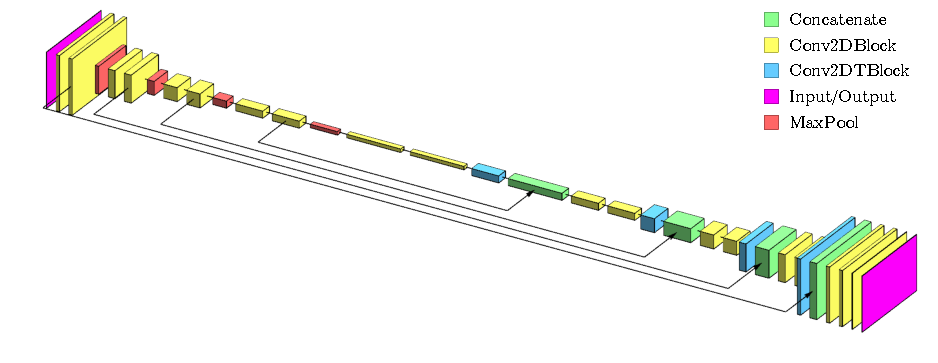
\includegraphics[width=\textwidth]{unet}
    \caption{The architecture of our final model. (The dimensions of the blocks correspond to the tensor shapes output by each layer.)}
    \label{fig:architecture}
\end{figure}

The training target was (as in \cite{YuKTJ16}) the mean squared error of the separated magnitude spectra reconstructed using the estimated masks:

\begin{gather}
    \label{eq:loss}
    J = \frac{1}{T \times F \times S} \sum_{i=1}^S \left\lVert \left| \mx{X}_i \right|  - \hat{\mx{M}}_i \circ \left| \mx{Y} \right| \right\rVert
\end{gather}

where $\left\lVert . \right\rVert$ denotes the Frobenius-norm of a matrix. It is important to note that this training target is superior to simply training for an ideal mask, since in silent segments, the perfect mask is underdetermined. Because of this, the value of the masks is irrelevant during these time periods, and the actual audible output should be considered, as in the above $J$ loss.

The final loss was calculated in a permutation-invariant way, which was the main idea of the \textit{permutation invariant training} (PIT) presented in \cite{YuKTJ16}. Simply put, a long-standing problem in supervised speech separation training was that the network had to learn which of its outputs are compared to which speaker channel during loss calculation. This makes the model unnecessarily hard to train. When using PIT instead, the loss is calculated for every possible permutation of pairs between output and reference channels. We had to implement the permutation-invariant loss function and the \eqref{eq:loss} calculation in Keras ourselves.

The training of the final model took about 10 hours on an Nvidia GTX 1070 GPU. The Adam optimization algorithm was used with early stopping based on the validation set results.

\section{Hyperparameter-tuning}
The final model was the result of a considerable amount of hyperparameter-tuning. First we based our model on those of \cite{YuKTJ16} and \cite{Chandna17}: a contractive convolutional part followed by densely connected layers. These models performed poorly in our experience on our 5 sec long audio segments: we suspect that this is at least partly due to the fact that the last layers destroy the spatial structure output by the previous convolutional layers. Also, these models have an unnecessarily large number of parameters. On our second try we tried a fully convolutional network like the final model, but with no skip connections. The results from this network was better (around 7 dB SDR), but adding the skip connections and thus building an U-Net-like architecture proved the best of all approaches. We trained the network every time with and without a final softmax activation layer based on the considerations discussed above. In the final model it did not affect the training loss values significantly, but the SDR values during testing were better by about 1.5 dB when using the softmax layer, and the subjective results were also much better. Because of this, we chose to include the softmax layer in our final network. This result was a bit surprising given that assuming sum of the magnitude-masks to be identity is conceptually flawed, as discussed above. A more detailed hyperparameter-tuning was not possible for us due to the long training time of the model.

\section{Test results}
The performance of the trained model was evaluated on the separate test set generated previously. An example result is illustrated on Figure \ref{fig:spectrograms} with spectrograms. For an objective measure the signal-to-distortion ratio (SDR) \cite{Vincent06} was calculated for the test set. For reference, the SDR values of the mixed (non-separated) signals and signals separated using an Ideal Ratio Mask (IRM) \cite{Wang14} were also computed: these can be considered the two possible extremes in performance. The average SDR of our model's output was $9.24\,\mathrm{dB}$ which is quite good considering the reference values $0.12\,\mathrm{dB}$ and $12.02\,\mathrm{dB}$. While \cite{YuKTJ16} used a different dataset, our SDR values compare well to their results. A non-representative, subjective auditory evaluation was also performed on the separated channels output by our model: while the separated signals are not perfect, none of the test subjects had any problem understanding the separated speech signals, which was not true for the mixed (non-separated) signals. 

\begin{figure}
    \centering
    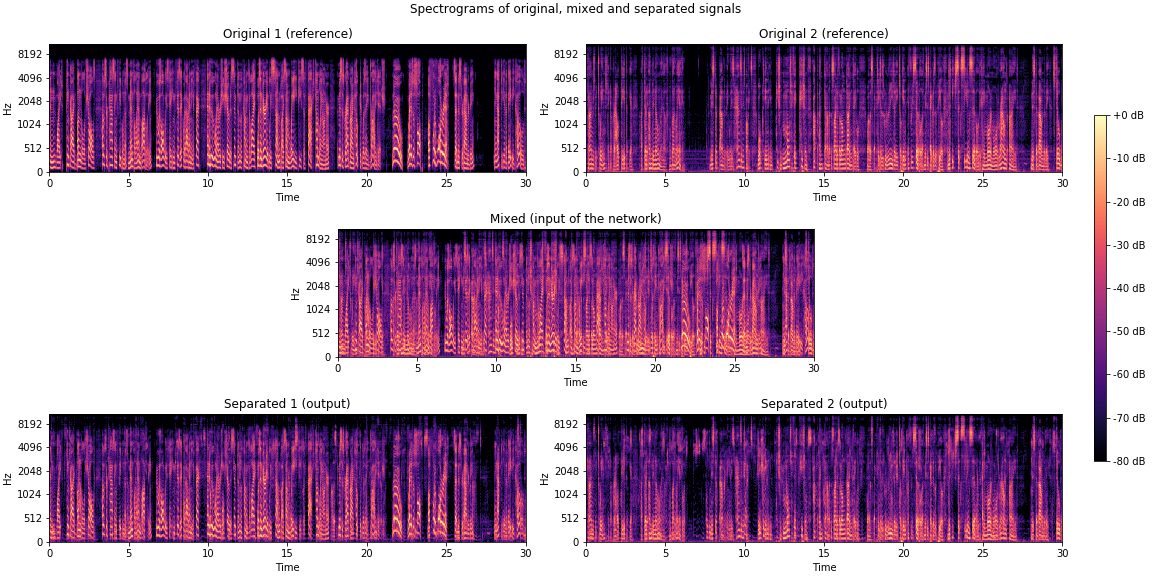
\includegraphics[width=\textwidth]{spectrograms.png}
    \caption{A separation example with spectrograms as an illustration of the process.}
    \label{fig:spectrograms}
\end{figure}
\section{Speaker tracing}
The previously discussed, improved loss function makes training the model much more successful, but introduces the problem that the network outputs might switch output channels between utterances. However, this can be eliminated using a traditional speaker-tracing algorithm. This was only alluded to in \cite{YuKTJ16}, but not realized. We implemented an algorithm for this based on \cite{Lilt04}. 20 Mel Frequency Cepstrum Coefficients were used as features, from which a set of feature vectors are calculated for each reconstructed speaker channel at every 5 sec segment:
\begin{gather}
    \mx{s}^j_i = \mathrm{MFCC}(\hat{\mx{x}}^j_i), \quad i=1,...,S,\,j=1,...,N
\end{gather}
where $N$ is the number of 5 sec segments that the original audio was separated into. The speaker tracing was done by calculating the negative generalized likelihood ratio for every possible permutation of outputs for consecutive segments. Considering the two-speaker case for simplicity, from four feature sets $\mx{s}_1^j$, $\mx{s}_2^j$, $\mx{s}_1^{j+1}$ and $\mx{s}_2^{j+1}$ and their pairwise unions
\begin{gather}
    \mx{s}_{11}^j = \mx{s}_1^j \cup \mx{s}_1^{j+1} \quad \mx{s}_{12}^j = \mx{s}_1^j \cup \mx{s}_2^{j+1} \\
    \mx{s}_{21}^j = \mx{s}_2^j \cup \mx{s}_1^{j+1} \quad \mx{s}_{22}^j = \mx{s}_2^j \cup \mx{s}_2^{j+1} \\
    j=1,...,N-1 \nonumber
\end{gather}
multivariate Gaussian distributions $\mx{s}_{k}^j \rightarrow (\mx{\mu}_k^j;\mx{\Sigma}_k^j)$ with $k\in \{1,2,11,12,21,11\}$ are estimated. The generalized likelihood ratio between a certain pairing of two consecutive outputs is:
\begin{gather}
    \mathrm{GLR}^j_{i,k} = \frac{L(\mx{s}^j_{ik} | (\mx{\mu}_{ik}^j;\mx{\Sigma}_{ik}^j))}{L(\mx{s}^j_{i} | (\mx{\mu}_{i}^j;\mx{\Sigma}_{i}^j)) L(\mx{s}^{j+1}_{k} | (\mx{\mu}_{k}^{j+1};\mx{\Sigma}_{k}^{j+1}))} \quad i,k = 1,...,S,\,j=1,...,N-1
\end{gather}
where $L$ is the likelihood of the data given the Gaussian model. This value gives the likelihood ratio of the two segments being generated by the same process compared to being generated by two different processes (e.g. being from the same speaker versus from two different speakers). In practice, the log likelihoods $\log(\mathrm{GLR}^j_{1,1})$ are used, since the likelihoods have very small numerical values for such high dimensional distributions, and the division can result in significant numerical errors. Considering again the two speaker-case, for the two possible pairings of outputs two distance metrics can be constructed based on the above $\mathrm{GLR}^j_{i,k}$ values:
\begin{align}
    d_{same}^j &= -\log(\mathrm{GLR}^j_{1,1}) -\log(\mathrm{GLR}^j_{2,2}) \\
    d_{switch}^j &= -\log(\mathrm{GLR}^j_{2,1}) -\log(\mathrm{GLR}^j_{1,2})
\end{align}
If $d_{same}^j>d_{switch}^j$, the outputs of the network were switched between segments $j$ and $j+1$, so these channels have to be switched during the reconstruction of the full-length audio channels.

\section{Conclusion and perspectives}
We used an U-Net-like deep neural network architecture for monaural two-speaker separation. This approach was not found in relevant literature, but showed promising and usable results, while there is still room for improvement. Training on a larger dataset, preferably the WSJ0 \cite{wsj0} dataset used in \cite{YuKTJ16} would be necessary for objective comparison of our model to the state of the art. Evaluating the model on unknown speakers or languages would be an interesting new angle, as well as varying the relative signal levels of the channels before constructing the mixed signals. A more detailed hyperparameter-optimization would also be in order. Using not only the magnitude but also the phase spectra during separation should also be investigated: it would probably further improve model performance.
\subsubsection*{Acknowledgments}

We would like to thank Dr. Tamás Gábor Csapó from TMIT for the consultations before submitting our work for milestones, as well as Áron Ritter and Bence Sipos for the insightful discussions and kindly provided GPU-time.

\bibliographystyle{unsrt}
\bibliography{bibliography}

\end{document}
